% !TEX TS-program = pdflatex
\documentclass[11pt]{article}

% -------------------- Packages --------------------
\usepackage[a4paper,margin=1in]{geometry}
\usepackage{amsmath,amssymb}
\usepackage[T1]{fontenc}
\usepackage{lmodern}
\usepackage{xcolor}
\usepackage{tcolorbox}
\tcbuselibrary{skins,breakable}
\usepackage{enumitem}
\usepackage{hyperref}
\usepackage{tikz}
\usetikzlibrary{calc,angles,quotes,arrows.meta}

\pagestyle{empty}

% -------------------- Dark Theme Colors --------------------
\definecolor{bg}{HTML}{000000}
\definecolor{pairbg}{HTML}{121212}
\definecolor{solbg}{HTML}{0A0A0A}
\definecolor{border}{HTML}{2A2A2A}
\definecolor{text}{HTML}{FFFFFF}
\definecolor{muted}{HTML}{C9CDD3}
\definecolor{gold}{HTML}{FFD700}
\definecolor{green}{HTML}{4ADE80}
\definecolor{cyan}{HTML}{38BDF8}

\pagecolor{bg}
\color{text}

\hypersetup{
  colorlinks=true,
  linkcolor=cyan,
  urlcolor=cyan
}

\setlength{\parindent}{0pt}
\setlength{\parskip}{10pt}

% Help LaTeX avoid overfull lines globally
\sloppy
\setlength{\emergencystretch}{3em}

\setlist[itemize]{left=1.4em,itemsep=6pt,topsep=6pt}
\setlist[enumerate]{left=1.6em,itemsep=4pt,topsep=4pt}

% -------------------- tcolorbox Base --------------------
\tcbset{
  enhanced,
  breakable,
  arc=12pt,
  boxrule=0.8pt,
  left=14pt,right=14pt,top=12pt,bottom=12pt
}

\newtcolorbox{QAPair}[1]{%
  colback=pairbg,
  colbacklower=solbg,
  colframe=border,
  coltext=text,
  title=\textcolor{gold}{\bfseries #1},
  fonttitle=\bfseries,
  coltitle=text,
  segmentation style={draw=border, dashed, line width=0.6pt},
  before upper=\raggedright,
  before lower=\raggedright
}

\newtcolorbox{QuickBox}{%
  colback=pairbg,
  colframe=cyan,
  coltext=text,
  fontupper=\color{text}\raggedright,
  borderline north={4pt}{0pt}{cyan},
  arc=14pt,
  boxrule=0.8pt
}

% Each MCQ in its own box
\newtcolorbox{MCQBox}[1]{%
  colback=solbg,
  colframe=border,
  coltext=text,
  arc=14pt,
  boxrule=0.8pt,
  left=12pt,right=12pt,top=10pt,bottom=10pt,
  breakable,
  title=\textcolor{gold}{\bfseries #1},
  fonttitle=\bfseries,
  before upper=\raggedright
}

% Helper for step headings
\newcommand{\Step}[1]{\textcolor{muted}{\textbf{Step #1:}}}

% Small centered diagram block (for step-by-step visuals)
\newenvironment{StepDiagram}{\par\medskip\begin{center}}{\end{center}\medskip}

% A tiny "equation diagram" (nice for 1-line algebra)
\newcommand{\EqDiagram}[1]{%
\begin{StepDiagram}
\begin{tikzpicture}
\node[draw=border, rounded corners=10pt, inner sep=8pt, text=text, align=left, text width=0.88\linewidth] {#1};
\end{tikzpicture}
\end{StepDiagram}
}

% --------- Normal-length blanks (replaces \dotfill) ----------
\newcommand{\Blank}[1][1.6cm]{%
  \tikz[baseline=-0.6ex]\draw[draw=text, line width=0.9pt] (0,0) -- (#1,0);
}

% TikZ styles
\tikzset{
  base/.style={draw=text, line width=0.9pt, line cap=round, line join=round},
  new/.style={draw=cyan, line width=1.2pt, line cap=round, line join=round},
  help/.style={draw=muted, dashed, line width=0.9pt},
  ang/.style={draw=gold, line width=1.0pt},
  dot/.style={circle, fill=text, inner sep=1.2pt},
  lab/.style={text=text, font=\small},
  labm/.style={text=muted, font=\small},
  % filled labels/captions to prevent clashes
  labf/.style={text=text, font=\small, fill=bg, fill opacity=0.90, text opacity=1, inner sep=1.6pt, rounded corners=2pt},
  cap/.style={text=muted, font=\small, fill=bg, fill opacity=0.92, text opacity=1, inner sep=1.8pt, rounded corners=3pt},
}

% -------------------- Mini-diagrams for MCQs --------------------
\newcommand{\MiniCenterDot}[1]{\node[dot] at (#1) {}; }

\newcommand{\MiniTangentOnePoint}{%
\begin{tikzpicture}[scale=0.78]
  \def\r{1.25}
  \coordinate (O) at (0,0);
  \coordinate (P) at (\r,0);
  \coordinate (A) at (\r,-1.2);
  \coordinate (B) at (\r, 1.2);
  \draw[base] (O) circle (\r);
  \draw[new] (O)--(P);
  \draw[new] (A)--(B);
  \MiniCenterDot{O} \MiniCenterDot{P}
  \node[labf] at ($(O)!0.55!(P)+(0,0.22)$) {$r$};
  \node[labf, anchor=west] at ($(P)+(0.08,0.20)$) {$P$};
  \node[cap, anchor=north] at (0,-1.55) {Tangent touches at one point.};
\end{tikzpicture}
}

\newcommand{\MiniRadiusPerpTangent}{%
\begin{tikzpicture}[scale=0.78]
  \def\r{1.25}
  \coordinate (O) at (0,0);
  \coordinate (P) at ({\r*cos(30)},{\r*sin(30)});
  \coordinate (X) at ($(P)+({-1.4*sin(30)},{ 1.4*cos(30)})$);
  \coordinate (Y) at ($(P)+({ 1.4*sin(30)},{-1.4*cos(30)})$);
  \draw[base] (O) circle (\r);
  \draw[new] (O)--(P);
  \draw[new] (X)--(Y);
  \MiniCenterDot{O} \MiniCenterDot{P}
  \node[labf] at ($(O)!0.55!(P)+(0.15,0.05)$) {$r$};
  \node[cap, anchor=north] at (0,-1.55) {$OP\perp$ tangent.};
\end{tikzpicture}
}

\newcommand{\MiniTwoTangentsFromExternal}{%
\begin{tikzpicture}[scale=0.78]
  \def\r{1.15}
  \coordinate (O) at (0,0);
  \coordinate (E) at (2.6,0);
  \pgfmathsetmacro{\d}{2.6}
  \pgfmathsetmacro{\px}{(\r*\r)/\d}
  \pgfmathsetmacro{\py}{(\r*sqrt(\d*\d-\r*\r))/\d}
  \coordinate (P) at (\px,\py);
  \coordinate (Q) at (\px,-\py);

  \draw[base] (O) circle (\r);
  \draw[new] (E)--(P);
  \draw[new] (E)--(Q);
  \draw[help] (O)--(P);
  \draw[help] (O)--(Q);

  \MiniCenterDot{O} \MiniCenterDot{E} \MiniCenterDot{P} \MiniCenterDot{Q}
  \node[labf, anchor=west] at ($(E)+(0.08,0.15)$) {$E$};
  \node[cap, anchor=north] at (0,-1.65) {Two tangents from external point.};
\end{tikzpicture}
}

\newcommand{\MiniTangentsAtDiameterEnds}{%
\begin{tikzpicture}[scale=0.78]
  \def\r{1.15}
  \coordinate (O) at (0,0);
  \coordinate (A) at (-\r,0);
  \coordinate (B) at ( \r,0);
  \draw[base] (O) circle (\r);
  \draw[new] (A)--(B);
  \draw[new] ($(A)+(0,-1.3)$) -- ($(A)+(0,1.3)$);
  \draw[new] ($(B)+(0,-1.3)$) -- ($(B)+(0,1.3)$);
  \MiniCenterDot{O} \MiniCenterDot{A} \MiniCenterDot{B}
  \node[cap, anchor=north] at (0,-1.65) {Tangents at ends of diameter are parallel.};
\end{tikzpicture}
}

\newcommand{\MiniDistanceBetweenParallelTangents}{%
\begin{tikzpicture}[scale=0.78]
  \def\r{1.15}
  \coordinate (O) at (0,0);
  \coordinate (A) at (-\r,0);
  \coordinate (B) at ( \r,0);
  \draw[base] (O) circle (\r);
  \draw[new] ($(A)+(0,-1.3)$) -- ($(A)+(0,1.3)$);
  \draw[new] ($(B)+(0,-1.3)$) -- ($(B)+(0,1.3)$);
  \draw[help,<->] ($(A)+(0,-1.05)$) -- ($(B)+(0,-1.05)$);
  \node[labf] at (0,-1.25) {$2r$};
  \MiniCenterDot{O}
  \node[cap, anchor=north] at (0,-1.65) {Distance $=2r$ (diameter).};
\end{tikzpicture}
}

\newcommand{\MiniExternalTouch}{%
\begin{tikzpicture}[scale=0.78]
  \def\rA{1.05}
  \def\rB{0.70}
  \coordinate (O) at (0,0);
  \coordinate (O2) at ({\rA+\rB},0);
  \draw[base] (O) circle (\rA);
  \draw[base] (O2) circle (\rB);
  \draw[new] (O)--(O2);
  \MiniCenterDot{O} \MiniCenterDot{O2}
  \node[cap, anchor=north] at (0.9,-1.55) {$OO'=r_1+r_2$};
\end{tikzpicture}
}

\newcommand{\MiniCentralAngle}{%
\begin{tikzpicture}[scale=0.78]
  \def\r{1.15}
  \coordinate (O) at (0,0);
  \coordinate (A) at ({\r*cos(130)},{\r*sin(130)});
  \coordinate (B) at ({\r*cos(30)},{\r*sin(30)});
  \draw[base] (O) circle (\r);
  \draw[new] (O)--(A);
  \draw[new] (O)--(B);
  \MiniCenterDot{O} \MiniCenterDot{A} \MiniCenterDot{B}
  \pic[ang, "$\theta$", angle radius=7mm, angle eccentricity=1.25,
    pic text options={fill=bg, inner sep=1pt, rounded corners=2pt}] {angle=B--O--A};
  \node[cap, anchor=north] at (0,-1.65) {Central angle at the centre.};
\end{tikzpicture}
}

\newcommand{\MiniAngleInSemicircle}{%
\begin{tikzpicture}[scale=0.78]
  \def\r{1.15}
  \coordinate (O) at (0,0);
  \coordinate (A) at (-\r,0);
  \coordinate (B) at ( \r,0);
  \coordinate (C) at ({\r*cos(70)},{\r*sin(70)});
  \draw[base] (O) circle (\r);
  \draw[new] (A)--(B);
  \draw[new] (A)--(C);
  \draw[new] (B)--(C);
  \MiniCenterDot{A} \MiniCenterDot{B} \MiniCenterDot{C}
  \pic[ang, "$90^\circ$", angle radius=6mm, angle eccentricity=1.2,
    pic text options={fill=bg, inner sep=1pt, rounded corners=2pt}] {angle=A--C--B};
  \node[cap, anchor=north] at (0,-1.65) {Angle in semicircle is right.};
\end{tikzpicture}
}

\newcommand{\MiniInscribedHalfCentral}{%
\begin{tikzpicture}[scale=0.78]
  \def\r{1.15}
  \coordinate (O) at (0,0);
  \coordinate (A) at ({\r*cos(150)},{\r*sin(150)});
  \coordinate (B) at ({\r*cos(50)},{\r*sin(50)});
  \coordinate (C) at ({\r*cos(300)},{\r*sin(300)});
  \draw[base] (O) circle (\r);
  \draw[new] (O)--(A);
  \draw[new] (O)--(B);
  \draw[new] (C)--(A);
  \draw[new] (C)--(B);
  \MiniCenterDot{O} \MiniCenterDot{C}
  \pic[ang, "$100^\circ$", angle radius=7mm, angle eccentricity=1.25,
    pic text options={fill=bg, inner sep=1pt, rounded corners=2pt}] {angle=B--O--A};
  \pic[ang, "$50^\circ$", angle radius=7mm, angle eccentricity=1.25,
    pic text options={fill=bg, inner sep=1pt, rounded corners=2pt}] {angle=A--C--B};
  \node[cap, anchor=north] at (0,-1.75) {Inscribed $=\frac12$ central (same arc).};
\end{tikzpicture}
}

\newcommand{\MiniMinorMajor}{%
\begin{tikzpicture}[scale=0.72]
  \begin{scope}[xshift=-1.6cm]
    \def\r{1.05}
    \coordinate (O) at (0,0);
    \draw[base] (O) circle (\r);
    \MiniCenterDot{O}
    \node[cap, anchor=north] at (0,-1.55) {Minor: $<180^\circ$};
  \end{scope}
  \begin{scope}[xshift=1.6cm]
    \def\r{1.05}
    \coordinate (O) at (0,0);
    \draw[base] (O) circle (\r);
    \MiniCenterDot{O}
    \node[cap, anchor=north] at (0,-1.55) {Major: $>180^\circ$};
  \end{scope}
\end{tikzpicture}
}

\newcommand{\MiniSameSegment}{%
\begin{tikzpicture}[scale=0.75]
  \def\r{1.15}
  \coordinate (O) at (0,0);
  \coordinate (A) at ({\r*cos(160)},{\r*sin(160)});
  \coordinate (B) at ({\r*cos(20)},{\r*sin(20)});
  \coordinate (C) at ({\r*cos(300)},{\r*sin(300)});
  \coordinate (D) at ({\r*cos(240)},{\r*sin(240)});
  \draw[base] (O) circle (\r);
  \draw[new] (A)--(B);
  \draw[new] (C)--(A);
  \draw[new] (C)--(B);
  \draw[new] (D)--(A);
  \draw[new] (D)--(B);
  \pic[ang, "$\alpha$", angle radius=5.5mm, angle eccentricity=1.25,
    pic text options={fill=bg, inner sep=1pt, rounded corners=2pt}] {angle=A--C--B};
  \pic[ang, "$\alpha$", angle radius=5.5mm, angle eccentricity=1.25,
    pic text options={fill=bg, inner sep=1pt, rounded corners=2pt}] {angle=A--D--B};
  \node[cap, anchor=north] at (0,-1.75) {Same segment $\Rightarrow$ equal angles.};
\end{tikzpicture}
}

\newcommand{\MiniCyclicOpp}{%
\begin{tikzpicture}[scale=0.75]
  \def\r{1.15}
  \coordinate (O) at (0,0);
  \coordinate (A) at ({\r*cos(120)},{\r*sin(120)});
  \coordinate (B) at ({\r*cos(30)},{\r*sin(30)});
  \coordinate (C) at ({\r*cos(300)},{\r*sin(300)});
  \coordinate (D) at ({\r*cos(210)},{\r*sin(210)});
  \draw[base] (O) circle (\r);
  \draw[new] (A)--(B)--(C)--(D)--cycle;
  \pic[ang, "$\alpha$", angle radius=5.5mm, angle eccentricity=1.2,
    pic text options={fill=bg, inner sep=1pt, rounded corners=2pt}] {angle=D--A--B};
  \pic[ang, "$180^\circ-\alpha$", angle radius=5.5mm, angle eccentricity=1.2,
    pic text options={fill=bg, inner sep=1pt, rounded corners=2pt}] {angle=B--C--D};
  \node[cap, anchor=north] at (0,-1.75) {Opposite angles sum to $180^\circ$.};
\end{tikzpicture}
}

\newcommand{\MiniCyclicExterior}{%
\begin{tikzpicture}[scale=0.75]
  \def\r{1.15}
  \coordinate (O) at (0,0);
  \coordinate (A) at ({\r*cos(125)},{\r*sin(125)});
  \coordinate (B) at ({\r*cos(35)},{\r*sin(35)});
  \coordinate (C) at ({\r*cos(300)},{\r*sin(300)});
  \coordinate (D) at ({\r*cos(215)},{\r*sin(215)});
  \coordinate (E) at ($(A)!1.35!(B)$);
  \draw[base] (O) circle (\r);
  \draw[new] (A)--(B)--(C)--(D)--cycle;
  \draw[new] (A)--(E);
  \pic[ang, "$\beta$", angle radius=5.5mm, angle eccentricity=1.25,
    pic text options={fill=bg, inner sep=1pt, rounded corners=2pt}] {angle=D--A--E};
  \pic[ang, "$\beta$", angle radius=5.5mm, angle eccentricity=1.25,
    pic text options={fill=bg, inner sep=1pt, rounded corners=2pt}] {angle=B--C--D};
  \node[cap, anchor=north] at (0,-1.75) {Exterior angle = opposite interior.};
\end{tikzpicture}
}

\newcommand{\MiniQuadrant}{%
\begin{tikzpicture}[scale=0.75]
  \def\r{1.15}
  \coordinate (O) at (0,0);
  \coordinate (A) at ({\r*cos(180)},{\r*sin(180)});
  \coordinate (B) at ({\r*cos(90)},{\r*sin(90)});
  \coordinate (C) at ({\r*cos(30)},{\r*sin(30)});
  \draw[base] (O) circle (\r);
  \draw[new] (O)--(A);
  \draw[new] (O)--(B);
  \draw[new] (C)--(A);
  \draw[new] (C)--(B);
  \pic[ang, "$90^\circ$", angle radius=6mm, angle eccentricity=1.2,
    pic text options={fill=bg, inner sep=1pt, rounded corners=2pt}] {angle=B--O--A};
  \pic[ang, "$45^\circ$", angle radius=6mm, angle eccentricity=1.2,
    pic text options={fill=bg, inner sep=1pt, rounded corners=2pt}] {angle=A--C--B};
  \node[cap, anchor=north] at (0,-1.75) {Quadrant: inscribed $45^\circ$.};
\end{tikzpicture}
}

% ============================================================
\begin{document}

\begin{center}
{\LARGE\bfseries \textcolor{gold}{Miscellaneous Exercise 10 --- Solutions}}\\[-2pt]
\end{center}

% ============================================================
% QUICK FORMULAS (clash-free: captions outside + filled labels)
\begin{QuickBox}
{\color{cyan}\bfseries Quick formulas (Tangents \& Angles in a Circle)}\par\medskip

\begin{itemize}

\item \textbf{Tangent at a point is perpendicular to the radius at that point.}

\begin{StepDiagram}
\begin{tikzpicture}[scale=1.05]
  \def\r{2.0}
  \coordinate (O) at (0,0);
  \coordinate (T) at ({\r*cos(20)},{\r*sin(20)});
  \coordinate (X) at ($(T)+({-1.8*sin(20)},{ 1.8*cos(20)})$);
  \coordinate (Y) at ($(T)+({ 1.8*sin(20)},{-1.8*cos(20)})$);

  \draw[base] (O) circle (\r);
  \draw[new] (O)--(T);
  \draw[new] (X)--(Y);

  \node[dot] at (O) {};
  \node[dot] at (T) {};

  \node[labf, anchor=south east] at ($(O)+(-0.05,-0.05)$) {$O$};
  \node[labf, anchor=west] at ($(T)+(0.10,0.05)$) {$P$};

  % right angle mark at P
  \draw[base] ($(T)+(-0.18,0)$) -- ($(T)+(-0.18,-0.18)$) -- ($(T)+(0,-0.18)$);

  \node[labf] at ($(O)!0.55!(T)+(0.20,0)$) {$OP=r$};
  \node[cap, anchor=north] at (0,-2.55) {$OP\perp$ tangent at $P$.};
\end{tikzpicture}
\end{StepDiagram}

\item \textbf{From an external point, exactly two tangents can be drawn, and their lengths are equal.}

\begin{StepDiagram}
\begin{tikzpicture}[scale=1.00]
  \def\r{1.8}
  \coordinate (O) at (0,0);
  \coordinate (E) at (3.6,0);

  \pgfmathsetmacro{\d}{3.6}
  \pgfmathsetmacro{\px}{(\r*\r)/\d}
  \pgfmathsetmacro{\py}{(\r*sqrt(\d*\d-\r*\r))/\d}

  \coordinate (P) at (\px,\py);
  \coordinate (Q) at (\px,-\py);

  \draw[base] (O) circle (\r);
  \draw[new] (E)--(P);
  \draw[new] (E)--(Q);
  \draw[help] (O)--(P);
  \draw[help] (O)--(Q);

  \node[dot] at (O) {};
  \node[dot] at (E) {};
  \node[dot] at (P) {};
  \node[dot] at (Q) {};

  \node[labf, anchor=south] at ($(O)+(0,-0.10)$) {$O$};
  \node[labf, anchor=west] at ($(E)+(0.08,0.10)$) {$E$};
  \node[labf, anchor=south] at ($(P)+(0,0.05)$) {$P$};
  \node[labf, anchor=north] at ($(Q)+(0,-0.05)$) {$Q$};

  \node[labf] at ($(E)!0.52!(P)+(0.10,0.22)$) {$EP$};
  \node[labf] at ($(E)!0.52!(Q)+(0.10,-0.22)$) {$EQ$};

  \node[cap, anchor=north] at (0,-2.55) {$EP=EQ$ (tangents from the same external point).};
\end{tikzpicture}
\end{StepDiagram}

\item \textbf{Touching circles:}
\[
\text{External touch: } OO' = r_1+r_2
\qquad
\text{Internal touch: } OO' = |r_1-r_2|.
\]

\begin{StepDiagram}
\begin{tikzpicture}[scale=0.90]
  % External touch (top)
  \begin{scope}[yshift=2.25cm]
    \coordinate (O) at (0,0);
    \coordinate (O2) at (3.0,0);
    \def\rA{1.25}
    \def\rB{1.65}

    \draw[base] (O) circle (\rA);
    \draw[base] (O2) circle (\rB);
    \draw[new] (O)--(O2);
    \node[dot] at (O) {};
    \node[dot] at (O2) {};
    \node[labf, anchor=south] at ($(O)+(0,-0.10)$) {$O$};
    \node[labf, anchor=south] at ($(O2)+(0,-0.10)$) {$O'$};
    \node[cap, anchor=south] at (1.5,1.95) {External touch: $OO'=r_1+r_2$};
  \end{scope}

  % Internal touch (bottom)
  \begin{scope}[yshift=-2.35cm]
    \coordinate (O) at (0,0);
    \coordinate (O2) at (1.55,0);
    \def\rA{1.85}
    \def\rB{0.85}

    \draw[base] (O) circle (\rA);
    \draw[base] (O2) circle (\rB);
    \draw[new] (O)--(O2);
    \node[dot] at (O) {};
    \node[dot] at (O2) {};
    \node[labf, anchor=south] at ($(O)+(0,-0.10)$) {$O$};
    \node[labf, anchor=south] at ($(O2)+(0,-0.10)$) {$O'$};
    \node[cap, anchor=north] at (0.8,-2.20) {Internal touch: $OO'=|r_1-r_2|$};
  \end{scope}
\end{tikzpicture}
\end{StepDiagram}

\item \textbf{Inscribed angle theorem:} angle at circumference $=\dfrac12$ (central angle on the same arc).

\begin{StepDiagram}
\begin{tikzpicture}[scale=1.00]
  \def\r{2.0}
  \coordinate (O) at (0,0);
  \coordinate (A) at ({\r*cos(155)},{\r*sin(155)});
  \coordinate (B) at ({\r*cos(25)},{\r*sin(25)});
  \coordinate (C) at ({\r*cos(300)},{\r*sin(300)});

  \draw[base] (O) circle (\r);
  \draw[new] (O)--(A);
  \draw[new] (O)--(B);
  \draw[new] (C)--(A);
  \draw[new] (C)--(B);

  \node[dot] at (O) {};
  \node[dot] at (A) {};
  \node[dot] at (B) {};
  \node[dot] at (C) {};

  \node[labf, anchor=north] at ($(O)+(0,-0.10)$) {$O$};
  \node[labf, anchor=east]  at ($(A)+(-0.10,0)$) {$A$};
  \node[labf, anchor=west]  at ($(B)+(0.10,0)$) {$B$};
  \node[labf, anchor=west]  at ($(C)+(0.10,0)$) {$C$};

  \pic[ang, "$\theta$", angle radius=9mm, angle eccentricity=1.25,
    pic text options={fill=bg, inner sep=1pt, rounded corners=2pt}] {angle=B--O--A};

  \pic[ang, "$\tfrac{\theta}{2}$", angle radius=9mm, angle eccentricity=1.25,
    pic text options={fill=bg, inner sep=1pt, rounded corners=2pt}] {angle=A--C--B};

  \node[cap, anchor=north] at (0,-2.55) {$\angle ACB=\dfrac12\angle AOB$ (same arc $AB$).};
\end{tikzpicture}
\end{StepDiagram}

\item \textbf{Cyclic quadrilateral:} opposite angles are supplementary, and exterior angle equals opposite interior angle.

\begin{StepDiagram}
\MiniCyclicOpp
\end{StepDiagram}

\item \textbf{Ptolemy's Theorem (cyclic quadrilateral):}
\[
AC\cdot BD = AB\cdot CD + BC\cdot DA.
\]

\begin{StepDiagram}
\begin{tikzpicture}[scale=0.95]
  \def\r{1.9}
  \coordinate (O) at (0,0);
  \coordinate (A) at ({\r*cos(125)},{\r*sin(125)});
  \coordinate (B) at ({\r*cos(35)},{\r*sin(35)});
  \coordinate (C) at ({\r*cos(300)},{\r*sin(300)});
  \coordinate (D) at ({\r*cos(215)},{\r*sin(215)});

  \draw[base] (O) circle (\r);
  \draw[new] (A)--(B)--(C)--(D)--cycle;
  \draw[new] (A)--(C);
  \draw[new] (B)--(D);

  \node[dot] at (A) {};
  \node[dot] at (B) {};
  \node[dot] at (C) {};
  \node[dot] at (D) {};

  \node[labf, anchor=south] at ($(A)+(0,0.08)$) {$A$};
  \node[labf, anchor=south] at ($(B)+(0,0.08)$) {$B$};
  \node[labf, anchor=north] at ($(C)+(0,-0.08)$) {$C$};
  \node[labf, anchor=north] at ($(D)+(0,-0.08)$) {$D$};

  \node[cap, anchor=north] at (0,-2.45) {In cyclic $ABCD$: $AC\cdot BD = AB\cdot CD + BC\cdot DA$.};
\end{tikzpicture}
\end{StepDiagram}

\end{itemize}
\end{QuickBox}

% ============================================================
% Q1 (MCQs) - each MCQ in its own box + diagram
\begin{QAPair}{Question 1 (MCQs)}
\textcolor{gold}{\bfseries Question:}
Encircle the correct option in each MCQ.\\
\tcblower
\textcolor{green}{\bfseries Answers (each MCQ in a separate box):}

\begin{MCQBox}{MCQ (i)}
A tangent line touches the circle at \Blank[1.2cm] point(s).\\
(a) 1 \quad (b) 2 \quad (c) 3 \quad (d) 4\\
\textbf{Answer: (a) 1}
\begin{center}\MiniTangentOnePoint\end{center}
\end{MCQBox}

\begin{MCQBox}{MCQ (ii)}
A tangent line is \Blank[1.6cm] to radial segment.\\
(a) parallel \quad (b) equal \quad (c) perpendicular \quad (d) similar\\
\textbf{Answer: (c) perpendicular}
\begin{center}\MiniRadiusPerpTangent\end{center}
\end{MCQBox}

\begin{MCQBox}{MCQ (iii)}
How many tangents can be drawn on the circle from a point outside the circle?\\
(a) 1 \quad (b) 2 \quad (c) 3 \quad (d) infinite\\
\textbf{Answer: (b) 2}
\begin{center}\MiniTwoTangentsFromExternal\end{center}
\end{MCQBox}

\begin{MCQBox}{MCQ (iv)}
If two tangents are drawn on both ends of diameter of a circle, they are:\\
(a) perpendicular \quad (b) parallel \quad (c) intersecting \quad (d) none\\
\textbf{Answer: (b) parallel}
\begin{center}\MiniTangentsAtDiameterEnds\end{center}
\end{MCQBox}

\begin{MCQBox}{MCQ (v)}
Given radius of a circle is $4$ cm. The distance between two tangents drawn at the outer ends of diameter is:\\
(a) 2 cm \quad (b) 4 cm \quad (c) 6 cm \quad (d) 8 cm\\
\textbf{Answer: (d) 8 cm}
\begin{center}\MiniDistanceBetweenParallelTangents\end{center}
\end{MCQBox}

\begin{MCQBox}{MCQ (vi)}
How many tangents can be drawn on the circle from a point on the circle?\\
(a) 1 \quad (b) 2 \quad (c) none \quad (d) infinite\\
\textbf{Answer: (a) 1}
\begin{center}\MiniTangentOnePoint\end{center}
\end{MCQBox}

\begin{MCQBox}{MCQ (vii)}
Two tangents drawn from a point outside the circle are:\\
(a) perpendicular \quad (b) parallel \quad (c) not congruent \quad (d) congruent\\
\textbf{Answer: (d) congruent}
\begin{center}\MiniTwoTangentsFromExternal\end{center}
\end{MCQBox}

\begin{MCQBox}{MCQ (viii)}
If two circles touch externally, the distance between their centres is equal to sum of \Blank[1.2cm] of both circles.\\
(a) radii \quad (b) diameters \quad (c) circumferences \quad (d) area\\
\textbf{Answer: (a) radii}
\begin{center}\MiniExternalTouch\end{center}
\end{MCQBox}

\begin{MCQBox}{MCQ (ix)}
If two congruent circles touch externally, the distance between their centres is equal to \Blank[1.2cm] of a circle.\\
(a) radius \quad (b) diameter \quad (c) chord \quad (d) sector\\
\textbf{Answer: (b) diameter}
\begin{center}\MiniExternalTouch\end{center}
\end{MCQBox}

\begin{MCQBox}{MCQ (x)}
If two circles of radii $1.4$ cm and $2.5$ cm touch internally, the distance between their centres is equal to:\\
(a) 1.4 cm \quad (b) 2.5 cm \quad (c) 1.1 cm \quad (d) 3.9 cm\\
\textbf{Answer: (c) 1.1 cm}
\begin{center}
\begin{tikzpicture}[scale=0.90]
  \def\rA{1.65}
  \def\rB{0.95}
  \coordinate (O) at (0,0);
  \coordinate (O2) at (0.70,0);
  \draw[base] (O) circle (\rA);
  \draw[base] (O2) circle (\rB);
  \draw[new] (O)--(O2);
  \node[dot] at (O) {};
  \node[dot] at (O2) {};
  \node[cap, anchor=north] at (0.4,-2.15) {Internal touch: $OO'=|2.5-1.4|=1.1$};
\end{tikzpicture}
\end{center}
\end{MCQBox}

\begin{MCQBox}{MCQ (xi)}
Angle subtended by an arc at centre of circle is called \Blank[1.4cm] angle.\\
(a) reflex \quad (b) inscribed \quad (c) straight \quad (d) central\\
\textbf{Answer: (d) central}
\begin{center}\MiniCentralAngle\end{center}
\end{MCQBox}

\begin{MCQBox}{MCQ (xii)}
An angle inscribed in a half circle is:\\
(a) $0^\circ$ \quad (b) $45^\circ$ \quad (c) $90^\circ$ \quad (d) $180^\circ$\\
\textbf{Answer: (c) $90^\circ$}
\begin{center}\MiniAngleInSemicircle\end{center}
\end{MCQBox}

\begin{MCQBox}{MCQ (xiii)}
If central angle of minor arc of a circle is $100^\circ$, angle inscribed in corresponding minor arc is:\\
(a) $200^\circ$ \quad (b) $100^\circ$ \quad (c) $75^\circ$ \quad (d) $50^\circ$\\
\textbf{Answer: (d) $50^\circ$}
\begin{center}\MiniInscribedHalfCentral\end{center}
\end{MCQBox}

\begin{MCQBox}{MCQ (xiv)}
Central angle of minor arc of a circle is:\\
(a) less than $360^\circ$ \quad (b) less than $180^\circ$ \quad (c) greater than $360^\circ$ \quad (d) greater than $180^\circ$\\
\textbf{Answer: (b) less than $180^\circ$}
\begin{center}\MiniMinorMajor\end{center}
\end{MCQBox}

\begin{MCQBox}{MCQ (xv)}
Central angle of major arc of a circle is:\\
(a) less than $90^\circ$ \quad (b) less than $180^\circ$ \quad (c) greater than $90^\circ$ \quad (d) greater than $180^\circ$\\
\textbf{Answer: (d) greater than $180^\circ$}
\begin{center}\MiniMinorMajor\end{center}
\end{MCQBox}

\begin{MCQBox}{MCQ (xvi)}
All angles in a same segment of a circle are:\\
(a) equal \quad (b) acute \quad (c) obtuse \quad (d) supplementary\\
\textbf{Answer: (a) equal}
\begin{center}\MiniSameSegment\end{center}
\end{MCQBox}

\begin{MCQBox}{MCQ (xvii)}
If $ABCD$ is a cyclic quadrilateral and $\angle A=60^\circ$, then $\angle C=$ \Blank[1.2cm]\\
(a) $180^\circ$ \quad (b) $150^\circ$ \quad (c) $120^\circ$ \quad (d) $60^\circ$\\
\textbf{Answer: (c) $120^\circ$}
\begin{center}\MiniCyclicOpp\end{center}
\end{MCQBox}

\begin{MCQBox}{MCQ (xviii)}
An exterior angle of a cyclic quadrilateral is \Blank[1.5cm] the opposite interior angle.\\
(a) greater than \quad (b) less than \quad (c) equal to \quad (d) supplement of\\
\textbf{Answer: (c) equal to}
\begin{center}\MiniCyclicExterior\end{center}
\end{MCQBox}

\begin{MCQBox}{MCQ (xix)}
Inscribed angle of a quadrant of a circle is:\\
(a) $45^\circ$ \quad (b) $90^\circ$ \quad (c) $145^\circ$ \quad (d) $130^\circ$\\
\textbf{Answer: (a) $45^\circ$}
\begin{center}\MiniQuadrant\end{center}
\end{MCQBox}

\begin{MCQBox}{MCQ (xx)}
In the figure, angle $\theta$ is equal to:\\
(a) $45^\circ$ \quad (b) $94^\circ$ \quad (c) $23.5^\circ$ \quad (d) $47^\circ$\\
\textbf{Answer: (d) $47^\circ$}

\medskip
\Step{Reason:} Angles subtending the same chord are equal.

\begin{StepDiagram}
\begin{tikzpicture}[scale=1.05]
  \def\r{2.0}
  \coordinate (O) at (0,0);
  \coordinate (A) at ({\r*cos(115)},{\r*sin(115)});
  \coordinate (B) at ({\r*cos(40)},{\r*sin(40)});
  \coordinate (C) at ({\r*cos(310)},{\r*sin(310)});
  \coordinate (D) at ({\r*cos(220)},{\r*sin(220)});

  \draw[base] (O) circle (\r);
  \draw[new] (A)--(C);
  \draw[new] (A)--(D);
  \draw[new] (B)--(C);
  \draw[new] (B)--(D);

  \node[dot] at (A) {};
  \node[dot] at (B) {};
  \node[dot] at (C) {};
  \node[dot] at (D) {};

  \node[labf, anchor=south] at ($(A)+(0,0.08)$) {$A$};
  \node[labf, anchor=west]  at ($(B)+(0.10,0)$) {$B$};
  \node[labf, anchor=north] at ($(C)+(0,-0.08)$) {$C$};
  \node[labf, anchor=north] at ($(D)+(0,-0.08)$) {$D$};

  \pic[ang,"$\theta$",angle radius=7mm,angle eccentricity=1.25,
    pic text options={fill=bg, inner sep=1pt, rounded corners=2pt}] {angle=D--A--C};
  \pic[ang,"$47^\circ$",angle radius=7mm,angle eccentricity=1.25,
    pic text options={fill=bg, inner sep=1pt, rounded corners=2pt}] {angle=D--B--C};

  \node[cap, anchor=north] at (0,-2.55) {Same chord $DC \Rightarrow \angle DAC=\angle DBC=47^\circ$.};
\end{tikzpicture}
\end{StepDiagram}

\[
\boxed{\theta=47^\circ}
\]
\end{MCQBox}

\end{QAPair}

% ============================================================
% Q2 (diagram in EACH step)
\begin{QAPair}{Question 2}
\textcolor{gold}{\bfseries Question:}
In a circle whose diameter is $12$ cm, there is a central angle whose measure is $90^\circ$.
A chord joins the endpoints of the arc cut off by the angle. Find the length of the chord.
\tcblower
\textcolor{green}{\bfseries Answer:}\par

\Step{1} Diameter $=12$ cm $\Rightarrow$ radius $r=6$ cm.

\begin{StepDiagram}
\begin{tikzpicture}[scale=1.05]
  \coordinate (O) at (0,0);
  \def\r{2.1}
  \coordinate (L) at (-\r,0);
  \coordinate (R) at (\r,0);

  \draw[base] (O) circle (\r);
  \draw[new] (L)--(R);

  \node[dot] at (O) {};
  \node[dot] at (L) {};
  \node[dot] at (R) {};

  \node[labf, anchor=north] at ($(O)+(0,-0.10)$) {$O$};
  \node[labf, anchor=east]  at ($(L)+(-0.10,0)$) {$D_1$};
  \node[labf, anchor=west]  at ($(R)+(0.10,0)$) {$D_2$};

  \node[cap, anchor=north] at (0,-2.55) {Diameter $D_1D_2=12$ cm $\Rightarrow r=6$ cm.};
\end{tikzpicture}
\end{StepDiagram}

\Step{2} For central angle $\angle AOB=90^\circ$,
\[
AB=2r\sin\left(\frac{90^\circ}{2}\right)=2(6)\sin45^\circ=6\sqrt2\text{ cm}.
\]

\EqDiagram{$AB=2r\sin\!\left(\dfrac{\theta}{2}\right)=2(6)\sin45^\circ=6\sqrt2\text{ cm}$}

\begin{StepDiagram}
\begin{tikzpicture}[scale=1.05]
  \def\r{2.2}
  \coordinate (O) at (0,0);
  \coordinate (A) at ({\r*cos(135)},{\r*sin(135)});
  \coordinate (B) at ({\r*cos(45)},{\r*sin(45)});
  \coordinate (M) at ($(A)!0.5!(B)$);

  \draw[base] (O) circle (\r);
  \draw[new] (O)--(A);
  \draw[new] (O)--(B);
  \draw[new] (A)--(B);
  \draw[help] (O)--(M);

  \node[dot] at (O) {};
  \node[dot] at (A) {};
  \node[dot] at (B) {};
  \node[dot] at (M) {};

  \node[labf, anchor=north] at ($(O)+(0,-0.10)$) {$O$};
  \node[labf, anchor=east]  at ($(A)+(-0.10,0)$) {$A$};
  \node[labf, anchor=west]  at ($(B)+(0.10,0)$) {$B$};
  \node[labf, anchor=north] at ($(M)+(0,-0.10)$) {$M$};

  \pic[ang,"$90^\circ$",angle radius=9mm,angle eccentricity=1.18,
    pic text options={fill=bg, inner sep=1pt, rounded corners=2pt}] {angle=B--O--A};

  % right angle at M (OM ⟂ AB)
  \draw[base] ($(M)+(-0.18,0)$) -- ($(M)+(-0.18,0.18)$) -- ($(M)+(0,0.18)$);

  \node[cap, anchor=north] at (0,-2.65) {Drop $OM\perp AB$: half-chord $AM=r\sin45^\circ$.};
\end{tikzpicture}
\end{StepDiagram}

\[
\boxed{AB=6\sqrt2\text{ cm}}
\]
\end{QAPair}

% ============================================================
% Q3 (diagram in EACH step)
\begin{QAPair}{Question 3}
\textcolor{gold}{\bfseries Question:}
The diameter of a circle is $20$ cm long and a chord parallel to it is $12$ cm long.
Find the distance between the chord and the center of the circle.
\tcblower
\textcolor{green}{\bfseries Answer:}\par

\Step{1} Diameter $=20$ cm $\Rightarrow r=10$ cm, and half-chord $=\dfrac{12}{2}=6$ cm.

\begin{StepDiagram}
\begin{tikzpicture}[scale=1.00]
  \def\r{2.2}
  \coordinate (O) at (0,0);
  \coordinate (P) at (-1.45,1.05);
  \coordinate (Q) at ( 1.45,1.05);
  \coordinate (M) at (0,1.05);

  \draw[base] (O) circle (\r);
  \draw[new] (P)--(Q);
  \draw[help] (O)--(M);

  \node[dot] at (O) {};
  \node[dot] at (M) {};

  \node[labf, anchor=north] at ($(O)+(0,-0.10)$) {$O$};
  \node[labf, anchor=south] at ($(M)+(0,0.10)$) {$M$};

  \node[labf] at ($(P)!0.5!(M)+(0,0.28)$) {$6$};
  \node[labf] at ($(M)!0.5!(Q)+(0,0.28)$) {$6$};

  \node[cap, anchor=north] at (0,-2.55) {Chord $PQ=12$ cm $\Rightarrow$ half-chord $=6$ cm.};
\end{tikzpicture}
\end{StepDiagram}

\Step{2} Use the right triangle with hypotenuse $r$:
\[
d=\sqrt{r^2-\left(\frac{12}{2}\right)^2}
=\sqrt{10^2-6^2}
=\sqrt{64}=8\text{ cm}.
\]

\EqDiagram{$d=\sqrt{10^2-6^2}=\sqrt{64}=8\text{ cm}$}

\begin{StepDiagram}
\begin{tikzpicture}[scale=1.00]
  \coordinate (M) at (0,0);
  \coordinate (Q) at (2.2,0);
  \coordinate (O) at (0,1.7);

  \draw[new] (M)--(Q);
  \draw[new] (O)--(M);
  \draw[new] (O)--(Q);

  % right angle at M
  \draw[base] (-0.18,0) -- (-0.18,0.18) -- (0,0.18);

  \node[dot] at (O) {};
  \node[dot] at (M) {};
  \node[dot] at (Q) {};

  \node[labf, anchor=south] at ($(O)+(0,0.10)$) {$O$};
  \node[labf, anchor=north] at ($(M)+(0,-0.10)$) {$M$};
  \node[labf, anchor=west]  at ($(Q)+(0.10,0)$) {$Q$};

  \node[labf] at ($(M)!0.5!(Q)+(0,-0.30)$) {$6$};
  \node[labf] at ($(O)!0.5!(M)+(-0.35,0)$) {$d$};
  \node[labf] at ($(O)!0.5!(Q)+(0.22,0.06)$) {$r=10$};

  \node[cap, anchor=north] at (1.1,-0.95) {Right $\triangle OMQ$};
\end{tikzpicture}
\end{StepDiagram}

\[
\boxed{8\text{ cm}}
\]
\end{QAPair}

% ============================================================
% Q4 (diagram in EACH step)
\begin{QAPair}{Question 4}
\textcolor{gold}{\bfseries Question:}
In a cyclic quadrilateral $ABCD$ with sides $a=AB$, $b=BC$, $c=CD$, $d=DA$,
and diagonals $p=AC$ and $q=BD$, we can express diagonals in terms of the sides as:
\[
p\times q = (a\times c) + (b\times d).
\]
Find $q$ if $a=4$ cm, $b=5$ cm, $c=6$ cm, $d=3$ cm and $p=8$ cm.
\tcblower
\textcolor{green}{\bfseries Answer:}\par

\Step{1} Use Ptolemy’s Theorem:
\[
pq=ac+bd.
\]

\begin{StepDiagram}
\begin{tikzpicture}[scale=1.00]
  \def\r{2.2}
  \coordinate (O) at (0,0);
  \coordinate (A) at ({\r*cos(120)},{\r*sin(120)});
  \coordinate (B) at ({\r*cos(45)},{\r*sin(45)});
  \coordinate (C) at ({\r*cos(235)},{\r*sin(235)});
  \coordinate (D) at ({\r*cos(320)},{\r*sin(320)});

  \draw[base] (O) circle (\r);
  \draw[new] (A)--(B)--(D)--(C)--cycle;
  \draw[new] (A)--(D); % p
  \draw[new] (B)--(C); % q

  \node[dot] at (A) {};
  \node[dot] at (B) {};
  \node[dot] at (C) {};
  \node[dot] at (D) {};

  \node[labf, anchor=south] at ($(A)+(0,0.10)$) {$A$};
  \node[labf, anchor=south] at ($(B)+(0,0.10)$) {$B$};
  \node[labf, anchor=north] at ($(C)+(0,-0.10)$) {$C$};
  \node[labf, anchor=north] at ($(D)+(0,-0.10)$) {$D$};

  % Side labels (shifted outward, filled)
  \node[labf] at ($(A)!0.5!(B)+(0,0.30)$) {$a$};
  \node[labf] at ($(B)!0.5!(D)+(0.35,0)$) {$b$};
  \node[labf] at ($(C)!0.5!(D)+(0,-0.32)$) {$c$};
  \node[labf] at ($(A)!0.5!(C)+(-0.35,0)$) {$d$};

  % Diagonals labels (filled)
  \node[labf] at ($(A)!0.52!(D)+(0.20,-0.06)$) {$p$};
  \node[labf] at ($(B)!0.52!(C)+(-0.20,-0.06)$) {$q$};

  \node[cap, anchor=north] at (0,-2.85) {Cyclic $ABCD$ $\Rightarrow$ Ptolemy: $pq=ac+bd$.};
\end{tikzpicture}
\end{StepDiagram}

\Step{2} Substitute:
\[
pq=(4)(6)+(5)(3)=24+15=39.
\]

\EqDiagram{$pq=ac+bd=(4)(6)+(5)(3)=24+15=39$}

% (small partial diagram for the substitution step)
\begin{StepDiagram}
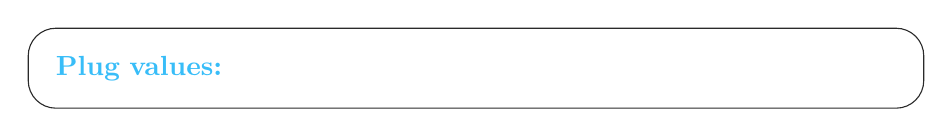
\begin{tikzpicture}
\node[draw=border, rounded corners=10pt, inner sep=10pt, text=text, align=left, text width=0.88\linewidth] {%
\textcolor{cyan}{\bfseries Plug values:}\quad
$ac=4\cdot 6=24,\;\; bd=5\cdot 3=15,\;\; ac+bd=39$};
\end{tikzpicture}
\end{StepDiagram}

\Step{3} Since $p=8$:
\[
q=\frac{39}{8}=4.875\text{ cm}.
\]

\EqDiagram{$q=\dfrac{39}{8}=4.875\text{ cm}$}

% (partial diagram for final division step)
\begin{StepDiagram}
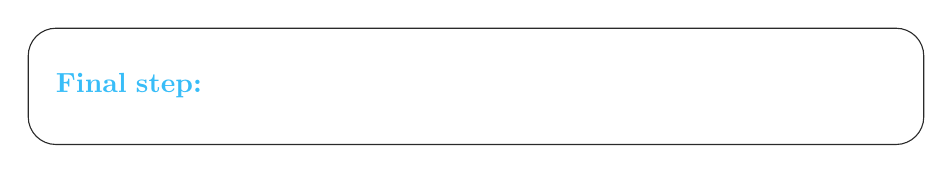
\begin{tikzpicture}
\node[draw=border, rounded corners=10pt, inner sep=10pt, text=text, align=left, text width=0.88\linewidth] {%
\textcolor{cyan}{\bfseries Final step:}\quad
$q=\dfrac{pq}{p}=\dfrac{39}{8}$};
\end{tikzpicture}
\end{StepDiagram}

\[
\boxed{q=\dfrac{39}{8}\text{ cm}\approx 4.875\text{ cm}}
\]
\end{QAPair}

\end{document}
